\section{Data analysis}
\label{data-analysis}

Before executing the algorithm, we performed a detailed analysis of the dataset.
Each dataset line is an event specific to an eCommerce store.
Altogether we have 109 950 743 records.
The first step was to identify if there were any null fields.
For this, we built a table with a single line, which shows the field count to null for each column, as shown in the table below.
\begin{center}
    \begin{tabular}{ | c | c | c | } 
        \hline
        \textbf{category\_code} & \textbf{brand} & \textbf{user\_session} \\ 
        \hline
        35 413 780 & 15 341 158 & 12 \\
        \hline
    \end{tabular}
\end{center}
We found many records with \textbf{brand} and \textbf{category\_code} at null and 12 records with \textbf{user\_session} to null.
We decided to remove these lines and not consider them for our recommendation system.
With these changes, we are left with a dataset of 68 650 184 records.

\subsection{Brand analysis}
For the analysis of brands, the quantity of products purchased and viewed from the various brands was counted.
Below are two graphs with this count:

\begin{figure}[H]
    \noindent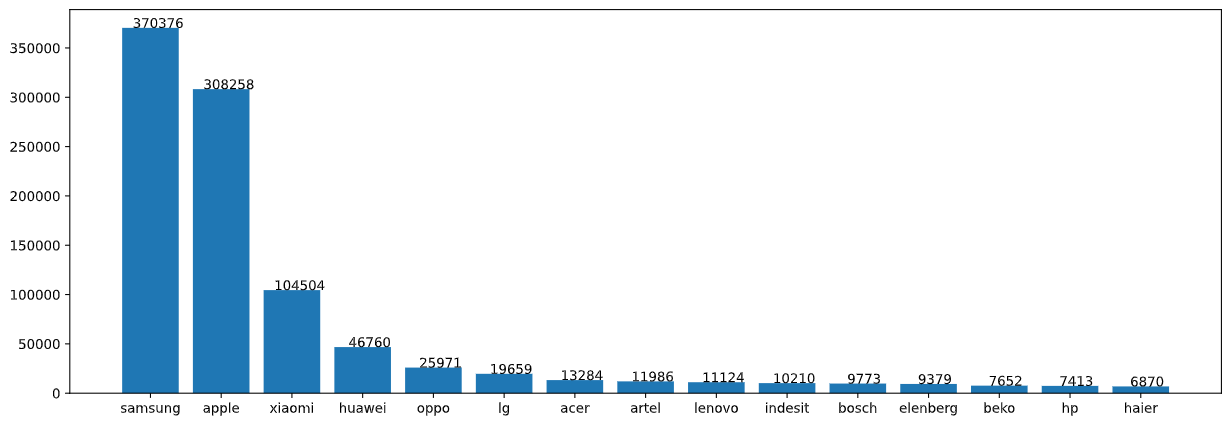
\includegraphics[width=\textwidth]{Count_brand_purchased.png}
    \caption{Count of brand products purchased.}
\end{figure}

\begin{figure}[H]
    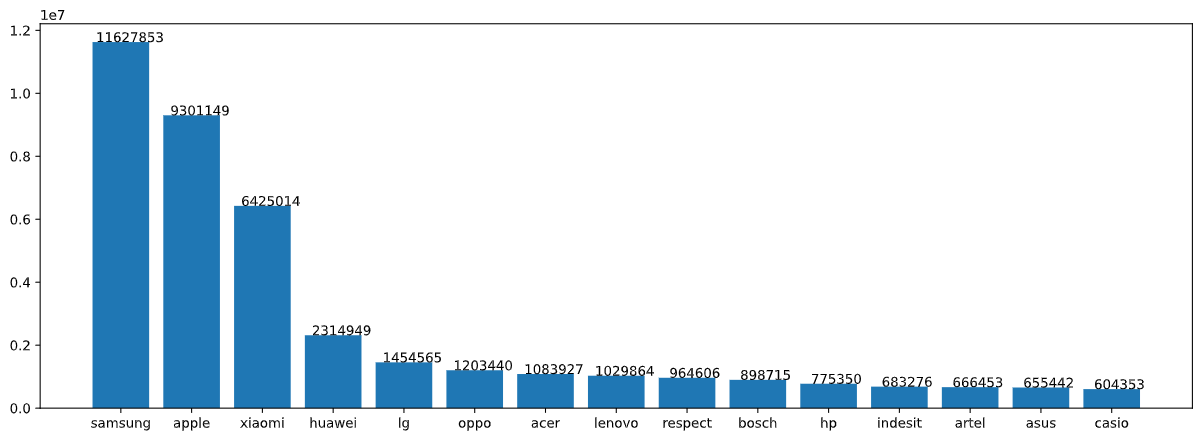
\includegraphics[width=\textwidth]{Count_brand_viewed.png}
    \caption{Count of brand products viewed.}
\end{figure}

As we can see, Samsung was the most viewed and purchased brand.
Apple and Xiaomi are also well represented in this digital store.
An interesting analysis that we can see now is the number of times a brand is seen to be purchased.

\begin{figure}[H]
    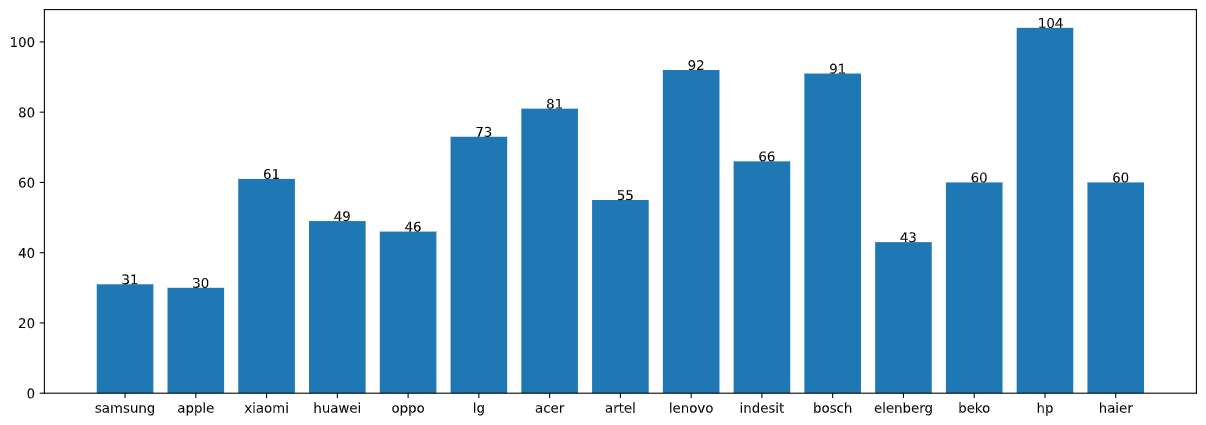
\includegraphics[width=\textwidth]{Brand_viewed_x_purchased.png}
    \caption{Number of times a brand is seen to be purchased.}
\end{figure}

We were able to observe that Samsung and Apple do not need to be seen very often to be purchased.
On the other hand, HP needs to be seen, on average, 104 times before it is purchased.

\subsection{Category analysis}
For the analysis of categories, the number of products by category that were purchased and viewed was analyzed.
Below are two graphs with this count:

\begin{figure}[H]
    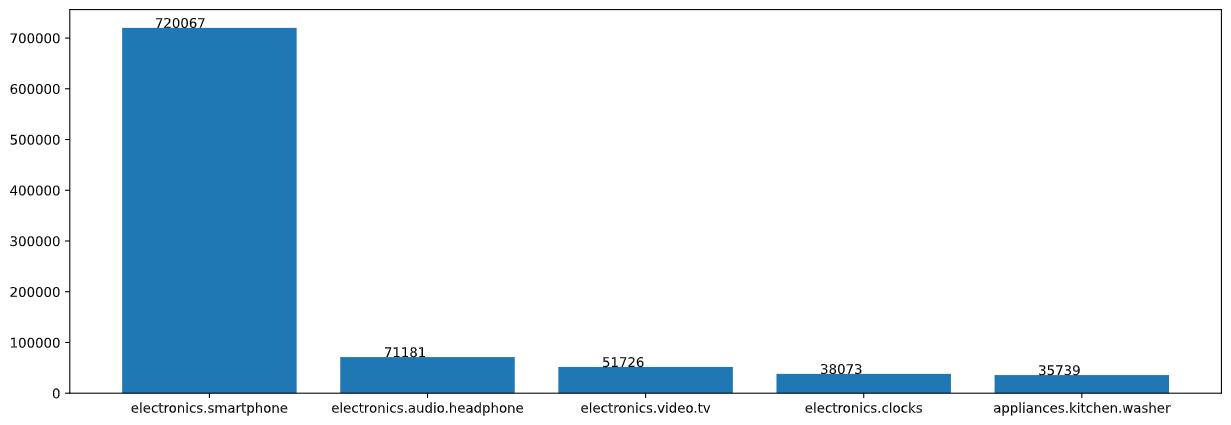
\includegraphics[width=\textwidth]{Count_category_purchased.png}
    \caption{Count of category products purchased.}
\end{figure}

\begin{figure}[H]
    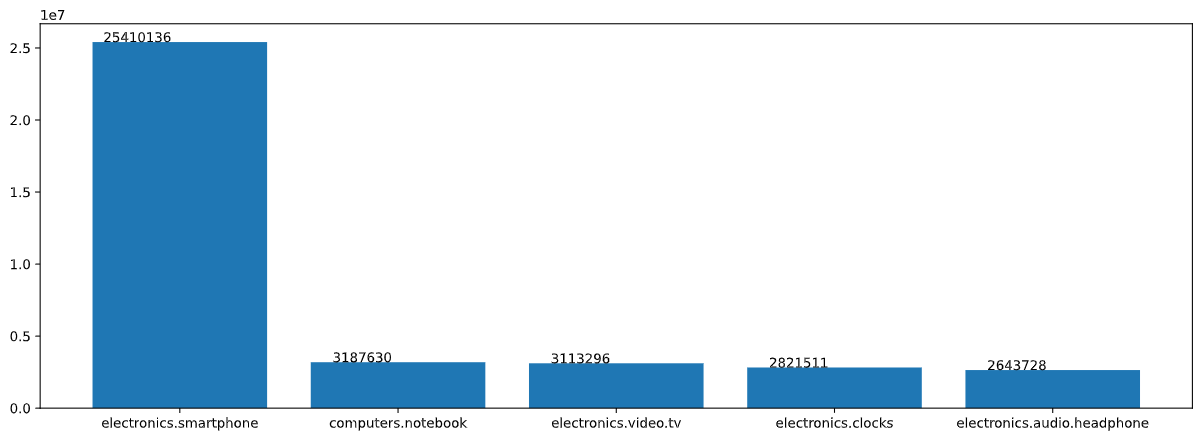
\includegraphics[width=\textwidth]{Count_category_viewed.png}
    \caption{Count of category products viewed.}
\end{figure}

As we can see, smartphones was the most viewed and purchased category, followed by far by computers, TVs, headphones, clocks and kitchen appliances.
An interesting analysis that we can see now is the number of times a category is seen to be purchased.

\begin{figure}[H]
    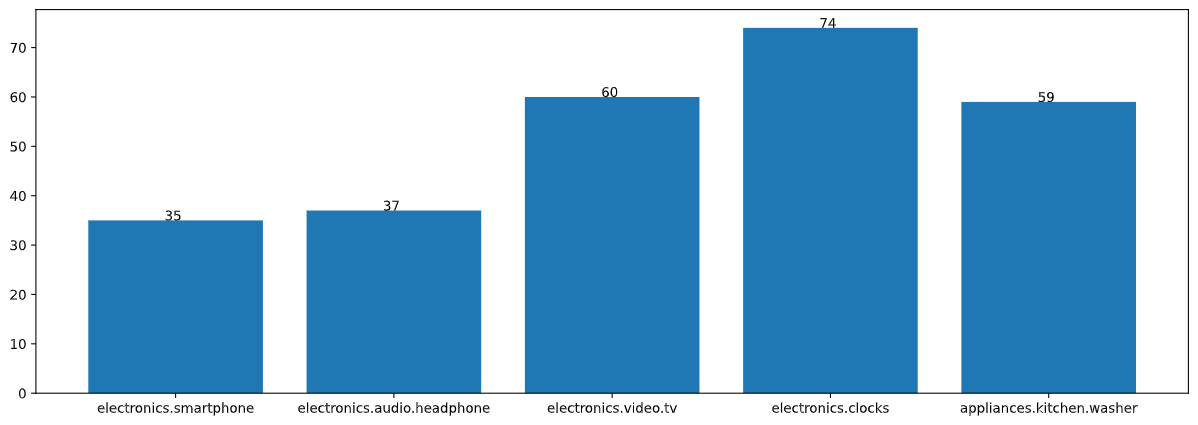
\includegraphics[width=\textwidth]{Category_viewed_x_purchased.png}
    \caption{Number of times a category is seen to be purchased.}
\end{figure}

We were able to observe that smartphones and headphones do not need to be seen very often to be purchased.
On the other hand, clocks needs to be seen, on average, 74 times before it is purchased.
